\section*{Part 1}
\subsection*{1a}
\begin{table}[h]
    \begin{tabular}{ll|ll}
        ~    & ~        & \multicolumn{2}{c}{Instruction} \\
        ~    & ~        & Single      & Multiple \\\hline
        \multirow{2}{*}{Data}         & Single   & SISD        & MISD     \\
        ~    & Multiple & SIMD        & MIMD     \\
    \end{tabular}
\end{table}

With MPI a single program (compiled source) is instantiated as multiple processes with different parameters.
Through MPI the processes send their computed results to some designated "master" process which consumes them into a single result for the entire program.
Therefore MPI fits under the MIMD category: there are multiple concurrent instruction streams, each working on their own data set.

\subsection*{1b}
If two processes reside on the same node, MPI can facilitate shared memory so that the processes can pass messages through it.

\subsection*{1c}
If two processes that need to communicate are not located on the same node,
they can not share memory, and must communcate over a network instead.

\subsection*{2a}
\subsubsection*{i}
The process with rank 0 has two jobs,
both computing its own slice of the sum formula,
then receving the results from the other processes and adding those up too.

Since all the processes are relatively equal they should all be done computing their part at about the same time.
At this point, process 0 must one by one receive the results in sequence.
The other processes this have to wait in a bottleneck for their turn to pass their message.
The process dependency tree would then look like a tree with one root, M mid-level nodes and N leaf nodes.

\subsubsection*{ii}
Process 0's computing part could be done by an extra process, making process 0 ready to receive sooner.
It would also be possible to parallelize the summing of contributions.
So for $N$ processes there would be some number $M$ of processes that each would sum $N / M$ contributions, and $1$ process that would finally sum the $M$ sums.

\section*{Part 2}
\subsection*{1c}
\subsubsection*{i}

\subsubsection*{ii}
alle:   init + rank + size
0:      P-1 * receive
~0:     send

3P + P-1 + 1 = 4P

\subsubsection*{iii}

\subsubsection*{iv}

\subsubsection*{v}
\begin{figure}[h]
    \centering
    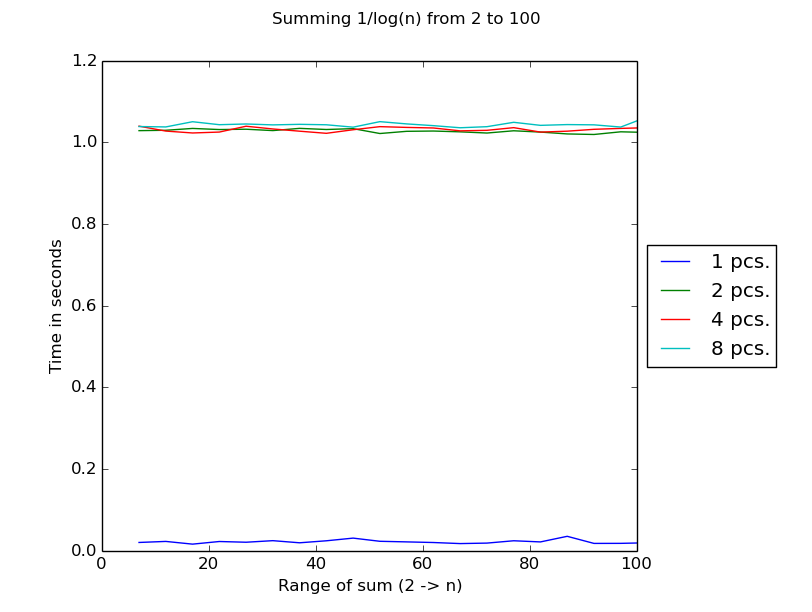
\includegraphics[width=0.32\textwidth]{10^2.png}
    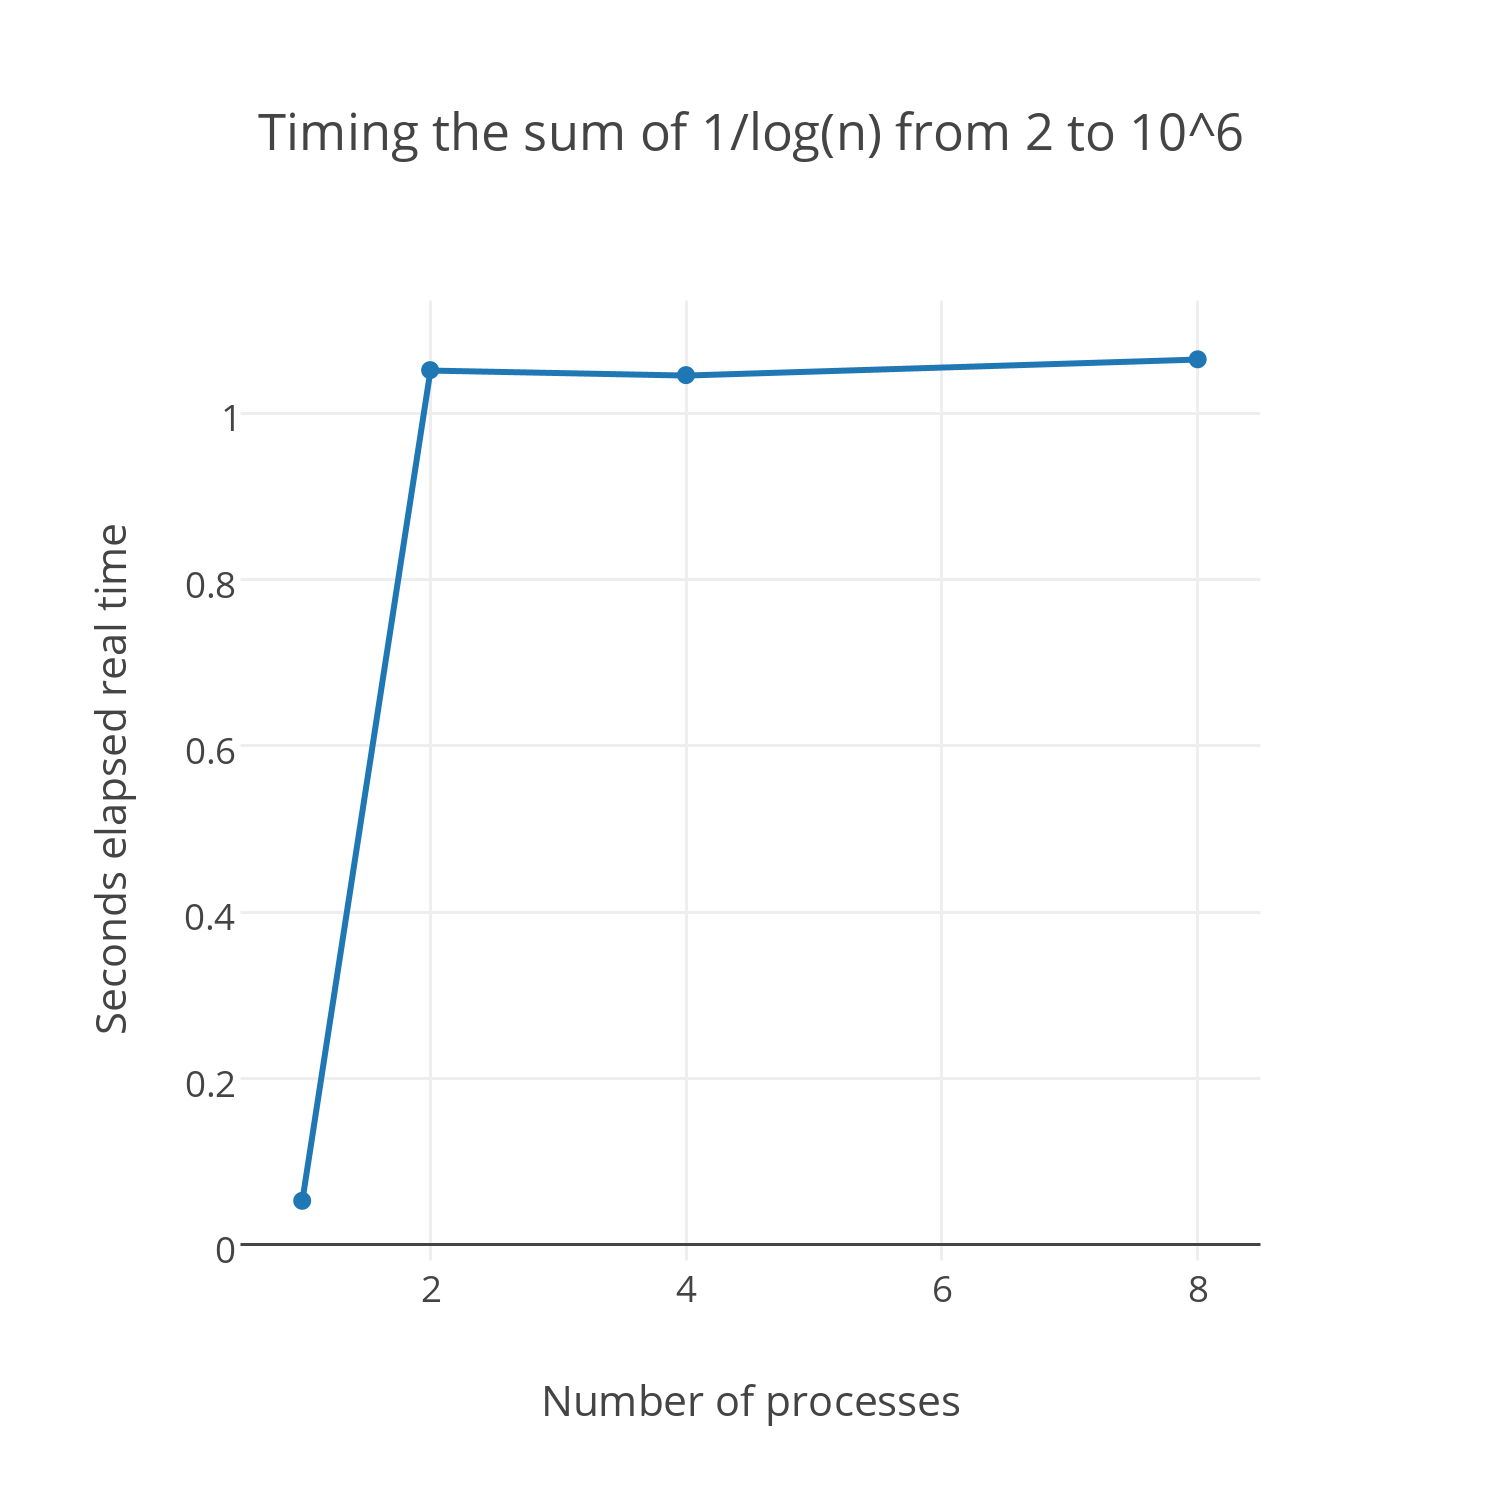
\includegraphics[width=0.32\textwidth]{10^6.png}
    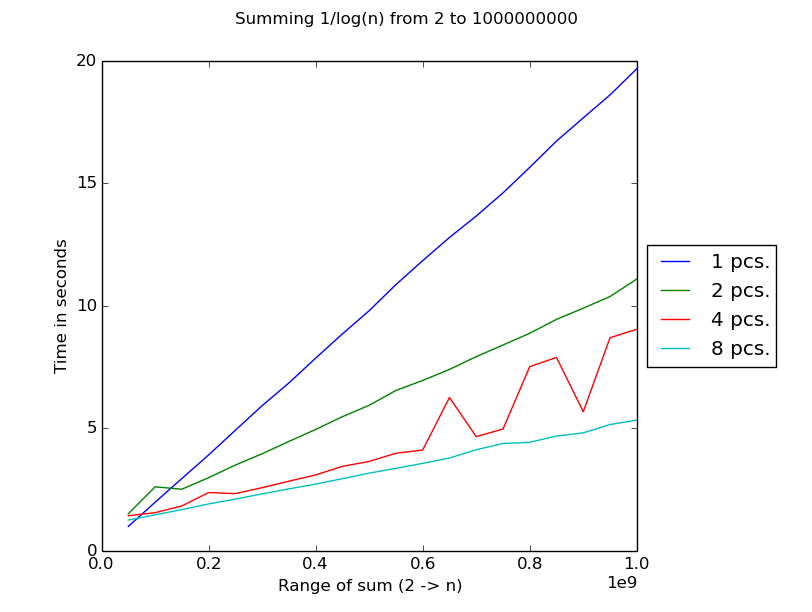
\includegraphics[width=0.32\textwidth]{10^9.png}
    \caption*{}
\end{figure}
We can see that the two smaller calculations are trivial for a single process,
and parallelizing it introduces overhead which takes more time.
For the largest calculation though, we can see that using parallel processes does improve the performance significantly.

%\begin{verbatim}
%    1       2       4       8
%^2  0.032   1.032   1.044   1.057
%^6  0.053   1.052   1.046   1.065
%^9  26.574  10.886  6.355   5.295
%\end{verbatim}
